Because it includes an on-shell Z boson as well as a b-jet and W from the top decay, tZ production represents an identical final state  to WZ + b-jet. This implies the possibility of matrix level interference between these two processes not accounted for in the Monte Carlo simulations, which consider the two processes independently. Truth level studies are performed in order to estimate the impact of these interference effects.    

In order to estimate the matrix level interference effects between tZ and WZ + b-jet, two different sets of simulations are produced using MadGraph 5 \cite{Madgraph} - one which simulates these two processes independently, and another where they are  produced simultaneously, such that interference effects are present. These two sets of samples are then compared, and the difference between them can be taken to represent any interference effects.

MadGraph simulations of 10,000 tZ and 10,000 WZ + b-jet events are produced, along with 20,000 events where both are present, in the fiducial region where three leptons and at least one jet are produced.  

A selection mimicking the preselection used in the main analysis is applied to the samples: The SS leptons are required to have $p_T>$20 GeV, and $>$10 GeV is required for the OS lepton. The associated b-jet is required to have $p_T>$25 GeV, and all physics objects are required to fall in a range of $|\eta|<$2.5. 

The kinematics of these samples after the selection has been applied are shown below:

\begin{figure}[H]
    \subfigure[]{\includegraphics[width=.47\linewidth]{tZInterference/lep1pt.eps}}%
    \subfigure[]{\includegraphics[width=.47\linewidth]{tZInterference/lep2pt.eps}}\\
    \subfigure[]{\includegraphics[width=.47\linewidth]{tZInterference/lep3pt.eps}}%
    \subfigure[]{\includegraphics[width=.47\linewidth]{tZInterference/lepPairMass23.eps}}\\
    \subfigure[]{\includegraphics[width=.47\linewidth]{tZInterference/mlvba.eps}}%
    \subfigure[]{\includegraphics[width=.47\linewidth]{tZInterference/btpt.eps}}\\
    \caption{Comparisons between (a) the $p_T$ of the lepton from the W, (b) and (c) show the $p_T$ of the lepton from the Z, (d)  the invariant mass of the Z-candidate, (e) the mass of the top candidate, and (f) the $p_T$ of the b-jet, for WZ and tZ events generated with interference effects (blue) and without interference effects (red).}
\end{figure}

The overall cross-section of the two methods agree within error, and no significant differences in the kinematic distributions are seen. It is therefore concluded that interference effects do not significantly impact the results.
